\section{La mise en place d'un cache pour les zones peuplées}
\subsection{Introduction}
Comme il a été possible de voir dans la partie~\ref{introSolutions}, la mise en place d'un cache pour les zones peuplées permettrait d'améliorer la réactivité dans l'état \textbf{W}(andering) (dans les zones denses). Un des avantages de cette solution était de s'intéresser à une partie qui n'avait pas encore été étudiée dans Blue Banana. Nous avons inséré un cache pour chaque nœud de l'environnement, celui-ci va fonctionner dans la continuité de liste des voisins d'un nœud. Nous expliquerons comment nous avons inséré le cache dans le code existant, les différentes stratégies que nous avons pu mettre en place et les différents paramètres qui vont influencer le fonctionnent du cache. Nous avons aussi permis l'utilisation du cache pour aider ses voisins quand ceux-ci cherchent des nœuds.
 
\subsection{Explications de la mise en place du cache}

\subsubsection{Le fonctionnement global et la mise en place du cache dans Blue Banana}
Le fonctionnement global du cache consiste à garder en mémoire un certain nombre de nœuds qui faisaient parti de l'ensemble des voisins. Ainsi, comme les mouvements de l'avatar sont désordonnés, il est possible qu'il retourne, dans un avenir proche, vers des nœuds qu'il vient de quitter. 
\par Sur la figure~\ref{cacheW}, les principales étapes du fonctionnement du cache sont représentées. Au départ le cache et la liste des voisins sont remplis de différents nœuds. A l'étape 2, le nœud courant (rouge) se déplace et trouve des nouveaux voisins, ceux-ci sont insérés dans sa liste des voisins. Deux nœuds sont alors déplacés vers le cache, ce qui pousse deux nœuds hors du cache. A la dernière étape, le nœud courant revient vers une zone qu'il connait (nous détaillerons après le mécanisme de recherche dans le cache) et il trouve deux nœuds dans son cache qui pourraient lui servir pour reconstruire son voisinage. Deux nœuds du cache sont alors insérés dans la liste des voisins du nœud courant, ce qui envoie deux nœuds de cette liste vers le cache. Dans cette exemple, plusieurs nœuds peuvent se déplacer en même temps, ce qui est le cas dans une des deux solutions de cache mise en place (l'autre solution ne renvoyant qu'un seul nœud).
	\begin{figure}[!h]
        \centering
        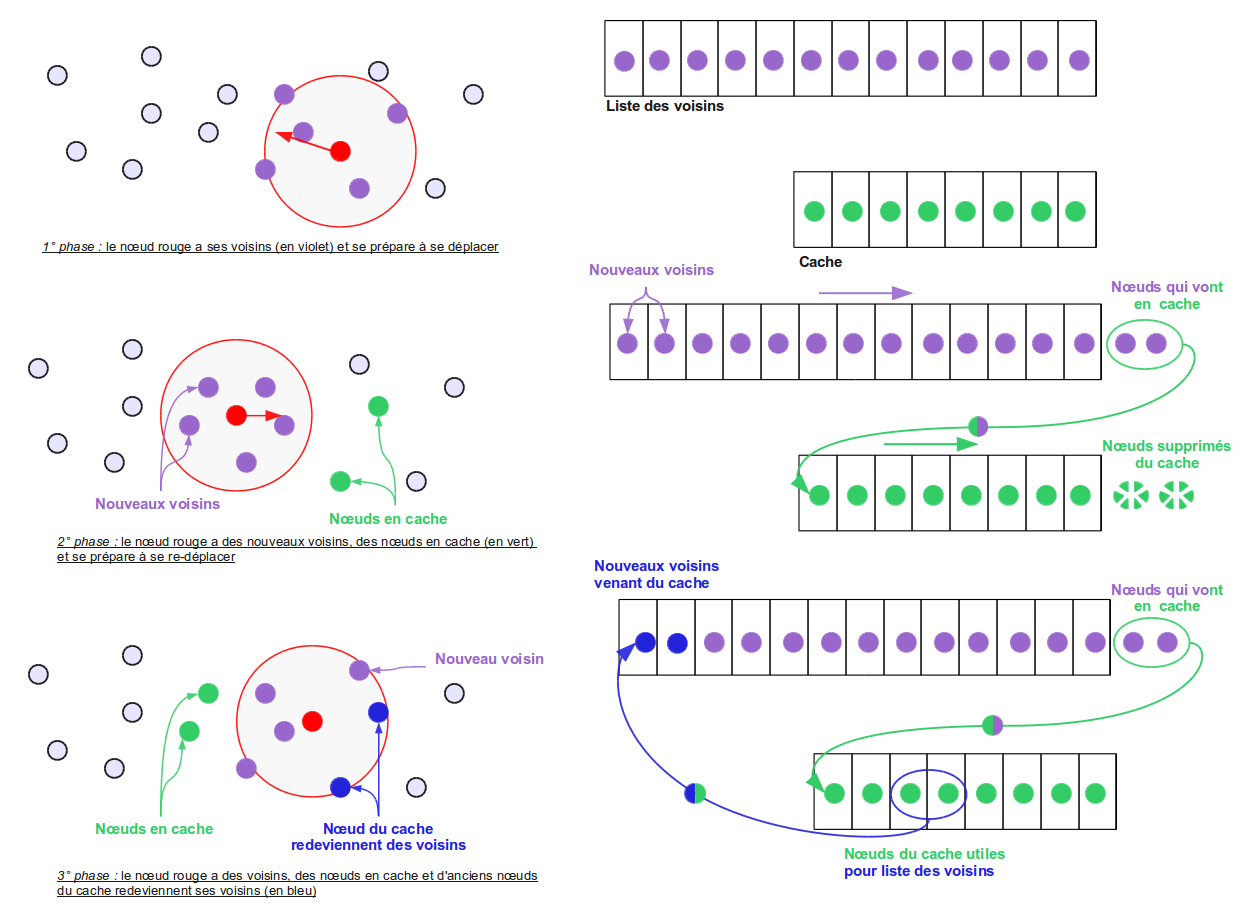
\includegraphics[scale=0.35]{./Ressources/Images/cacheWextends.png}
        \caption{Exemples du fonctionnement global du cache}
        \label{cacheW}
        \end{figure} 
\par Cette solution permet d'économiser des messages de découverte des voisins (SEARCH) dans le cas de changements de direction fréquents. Il doit aussi nous permettre d'économiser des messages de connexions et de déconnexion. Nous verrons dans la partie~\ref{resObsCache} les différents gains de la mise en place du cache, mais aussi les limites de celui-ci. Le cache est donc le prolongement de la liste des voisins pour nœud, mais contrairement à celui-ci, il n'est pas obligatoirement tenu à jour, car un nœud est ajouté dans le cache avec les dernières informations qui étaient disponibles dans la liste des voisins. 
\par Un système de mise à jour des données du cache a été mis en place, pour avoir des informations les plus exactes possibles sur chaque nœud. Mais ce système coûte cher en nombre de messages, et cela est encore plus vrai plus le cache est grand. Un mécanisme de datation des éléments du cache permet de savoir depuis quand date les informations de chacun. Ce mécanisme nous permet de contacter un nœud pour savoir s'il se trouve toujours à peu près au même endroit, et ainsi l'ajouter ou non à notre voisinage. Ces paramètres sont en option et nous verrons dans la partie~\ref{resObsCache} quelles sont les résultats de ces options et si elles sont toutes utiles ou non.

\subsubsection{Les différentes versions du cache}

Plusieurs versions, pour le fonctionnent du cache, ont été testées durant la phase de codage. Nous parlons ici de la gestion des données dans le cache et non de la recherche dans celui-ci qui se fera juste après. Au départ le cache était géré selon le principe \textit{First In First Out}. La gestion du cache se faisait sans tenir compte des mises à jour de certaines données qui peuvent avoir lieu lors d'une requête en échec vers un nœud du cache. Les données du nœud ayant trop bougé sont alors rafraichies dans le cache. Un autre gestion du cache en fonction de la localité temporelle des données est mise en place. Les tests sont réalisés avec cette version. Enfin une dernière gestion du cache en fonction de la localité spatiale a aussi été mise en place, ce qui permet de faire sortir du cache les nœuds les plus éloignés de la position actuelle du nœud.
\par Deux implémentations ont aussi été testées pour la recherche dans le cache, l'une renvoie un résultat et l'autre renvoie plusieurs nœud à ajouter. Les tests montrent que la deuxième implémentation donne de meilleurs résultats (voir chapitre~\ref{resObsCache}).


\subsubsection{La modification du code existant pour insérer la recherche dans le cache}

 Avant de regarder les algorithmes de recherche dans le cache, nous allons expliquer comment ils sont appelés et quelles sont les modifications introduites par rapport au code original. Lorsqu'un nœud rentre dans la fonction \textit{solipsisRecoverTopology} si le nœud est dans l'état \textbf{W}(andering) alors on passe dans la fonction \textit{MaintainTopology}, sinon on effectue le traitement normal. Nous pouvons voir ci-dessous une partie du code de la fonction \textit{MaintainCache}. Pour commencer, nous testons l'état de l'entité appelante, ensuite en fonction de la stratégie, nous faisons un traitement particulier. Nous nous concentrerons sur la stratégie de base qui ajoute un seul nœud. La fonction de recherche nous renvoie donc un résultat. S'il n'est pas nul et que sa date de mise à jour n'est pas trop ancienne, nous enlevons le nœud du cache, ajoutons le nœud à la liste des voisins et renvoyons 1 à la fonction appelante pour lui signifier que le traitement à été fait. Ensuite en fonction de la valeur de l'option \textit{contact\_node}, nous contactons ou non le nœud renvoyé par la fonction de recherche. Nous faisons ceci pour savoir s'il a beaucoup bougé depuis le dernier moment où nous l'avons vu. Nous retournons une valeur nulle pour signifier à la fonction appelante qu'aucun nœud n'a été ajouté et qu'elle peut faire le traitement de base.

\lstset{numbers=left,basicstyle=\scriptsize, numberstyle=\tiny, stepnumber=5, numbersep=5pt}

\lstinputlisting[title={Partie du code de la fonction MaintainCache},label={codeMaitainTopology}]{./Ressources/Documents/MaintainTopology.java}



\subsubsection{Les algorithmes de recherche dans le cache}
\par Nous allons expliquer de quelle façon les données sont recherchées dans le cache, et nous détaillerons les différentes pistes que nous avons testé. La méthode n°1 sélectionne les nœuds en terme de distance. L'idée est de récupérer les nœuds les plus proches de notre nouvelle position. Cette solution a été assez simple à mettre en place car il s'agit d'une simple comparaison de distance. 
\begin{table}[!h]
  \begin{center}
    \begin{tabular}{|c|c|c|c|}
      \hline
      N° & Critère de sélection & Avantages & Inconvénients\\
      \hline
      	1 & Comparaison distances & Simplicité & Distance~$\ne$~utile, aide pas enveloppe\\
      	2 & Aide enveloppe & + Enveloppe OK & - bon règles Solipsis\\
      	3 & Zone de connaissance & Simplicité & aide pas enveloppe\\
      \hline
    \end{tabular}
  \end{center}
  \label{tab:config1}
  \caption{Tableau montrant les valeurs utilisées pour la configuration n°1}
\end{table}


\par La méthode n°2 prend en compte la capacité d'un nœud à aider à refaire l'enveloppe connexe du nœud courant. Nous avons alors implémenté une solution qui rendait un résultat positif si un nœud dans le cache permettait de reconstruire l'enveloppe du nœud (voir la figure~\ref{schemaEnvelopCache}). Cette solution a même été agrémentée d'un test si le nœud faisait avancer positivement l'enveloppe connexe mais ne la reconstruisait pas immédiatement.

	\begin{figure}[!h]
        \centering
        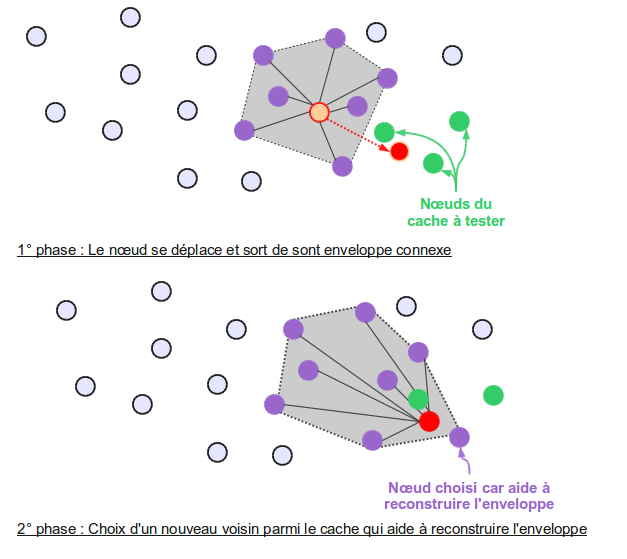
\includegraphics[scale=0.45]{./Ressources/Images/cacheReconstructEnvelop.png}
        \caption{Schéma montrant la solution de recherche dans le cache aidant à reconstruire l'enveloppe}
        \label{schemaEnvelopCache}
        \end{figure}
Le problème de la solution n°2 est qu'elle privilégiait l'enveloppe connexe à la propriété de \textit{Local Awareness}. Car nous pouvons nous retrouver dans la situation, comme dans la figure~\ref{schemaEnvelopCache}, où un nœud ne fait pas parti de la liste des voisins alors qu'il se trouve dans l'enveloppe connexe. Cette solution nous donnait donc des résultats, pour les propriétés de Solipsis, qui pouvaient être moins bons que la version sans le cache.  

\par La dernière méthode, la n°3, celle qui est retenu dans l'implémentation, ressemble à la solution n°1. Chaque nœud comporte une zone de connaissance, nous avons donc décidé de nous servir de cette dernière pour réaliser les conditions dans la fonction de recherche. La fonction de recherche regarde si un nœud du cache est dans la zone de connaissance du nœud courant. Si plusieurs correspondent un système pour choisir aléatoirement est mis en place, comme dans la fonction de recherche de voisin original. Une autre fonction qui recherche en prenant en compte la région géométrique a aussi été mise en place, les résultats sont équivalents à la version avec la zone de connaissance.

\subsubsection{La mise en place de l'aide aux voisins grâce au cache}

Le cache d'un nœud va donc lui servir pour connaitre son environnement plus rapidement, mais il pourrait aussi aider les voisins du nœud. Dans cette optique, l'aide aux voisins a été mise en place. Ceci permet au cache d'avoir une autre utilisation, ce qui pourrait permettre d'économiser quelques autres messages. 
\par Lorsqu'un nœud cherche des voisins, il envoie un message SEARCH (voir schéma~\ref{schemaHelpCache}). Il suffit donc d'insérer une recherche dans le cache au bon endroit dans la fonction de traitement de ce message. Nous insérons donc, dans la fonction \textit{processSearchMsg}, une fonction de recherche dans le cache. Le nœud va tout d'abord regarder dans sa liste des voisins et si aucun ne correspond, nous regardons dans le cache si un nœud peut correspondre à la requête. La recherche dans le cache se fait, de façon similaire à une recherche dans le cache pour un nœud local, en utilisant la zone de connaissance que l'on aura préalablement transmis dans le message.

	\begin{figure}[!h]
        \centering
        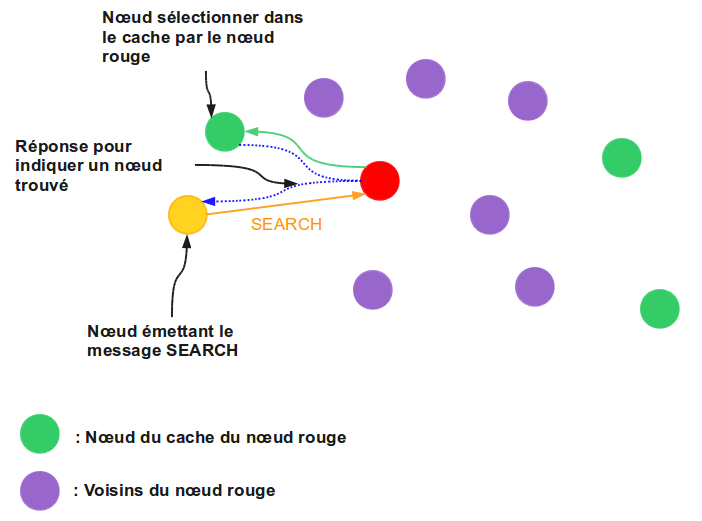
\includegraphics[scale=0.4]{./Ressources/Images/cacheHelp.png}
        \caption{Schéma montrant l'aide du cache pour le traitement d'un message SEARCH}
        \label{schemaHelpCache}
        \end{figure}

\subsection{Résultats et observations sur le cache}
\label{resObsCache}

Nous allons présenter les différents résultats sur le cache. Nous comparerons chaque version avec une version de base où l'on ne trouve ni cache ni préchargement, et avec une version avec le préchargement implémenté dans Blue Banana.
Les principales métriques pour comparer les différents résultats sont la cohérence de la topologie et le nombre de messages qui sont exprimés en fonction de la mobilité des avatars. Le calcul de la cohérence de la topologie consiste à mesurer, à chaque instant, le nombre de nœuds qui sont dans la zone de connaissance d'un autre nœud mais qui ne font pas parti des voisins de ce dernier.

\par Tout d'abord, nous allons regarder le nombre de cache Hit et Miss pour le cache normal. Il s'agit de voir le taux de réussite du cache et donc si ce mécanisme est souvent utlisé. Dans ces premiers résultats, le cache est configuré de tel sorte qu'il utilise l'aide aux voisins, mais qu'il ne contacte pas un nœud du cache s'il est trop vieux. Cette configuration ne va récupérer que les nœuds du cache qui sont très proches et qui ont été ajoutés au cache récemment (voir tableau ci dessous). La taille du cache correspond au nombre de nœud qu'il peut contenir, la limite de distance correspond à la distance à partir de laquelle nous ne récupèrerons pas le nœud. La limite de temps est la différence maximum qu'il doit y avoir entre le temps courant et la date de rafraichissement du nœud dans le cache (généralement l'ajout de celui-ci dans le cache). 
\begin{table}[!h]
  \begin{center}
    \begin{tabular}{|c|c|}
      \hline
      Paramètre & Valeur\\
      \hline
      Taille du cache & 25\\
      Limite de distance &  1500\\
      Limite de temps & 1500\\
      Contact Nœud & Faux\\
      Mise à jour du cache & Faux\\
      Aide aux voisins & Vrai\\
      \hline
    \end{tabular}
  \end{center}
  \label{tab:config1}
  \caption{Tableau montrant les valeurs utilisées pour la configuration n°1}
\end{table}


\par Nous pouvons voir que plus la mobilité augmente plus le nombre de cache Hit augmente et le nombre de cache Miss diminue (voir figure~\ref{courbesHitMiss:config1}). Cela est dû au fait que plus la mobilité augmente plus le cache aura des entrées récentes, car les nœuds vont changer de direction plus souvent et plus rapidement. Notre politique de cache ne prenant en compte que des nœuds récemment ajoutés au cache, les résultats en terme de cache Hit sont bien meilleurs. Nous pouvons aussi noter qu'il ya de moins en moins d'accès au cache car la somme des Hit et des Miss diminue, cela est du au fait que de plus en plus de nœuds sont dans un état \textbf{T}(ravelling). 

	\begin{figure}[!h]
        \centering
        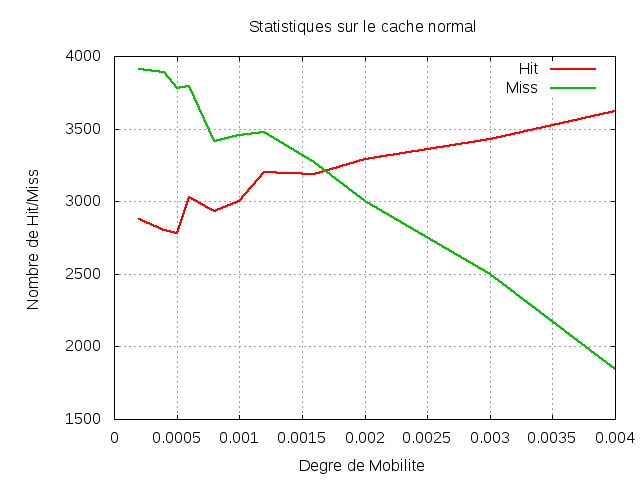
\includegraphics[scale=0.5]{../CacheCode/SolipsisPeersim/resultats/Courbes/Courbes_Final_Rapport/Cache_Stats_Normal.png}
        \caption{Schéma montrant les caches Hit et caches Miss pour le cache normal}
        \label{courbesHitMiss:config1}
        \end{figure}
\newpage
\par Ensuite nous pouvons observer le nombre de messages en fonction du degré de mobilité (voir figure~\ref{courbesNbMessCache:config1}). Les deux versions du cache vont permettre d'économiser des messages car lors d'un cache Hit nous ne faisons pas le traitement de base qui provoquait l'envoie d'un message. Le traitement du cache se fait sans coût en terme de message. Si l'on fait le traitement de base après le passage dans le cache, un gain en nombre de message sera tout de même réalisé. Ce gain résulte du fait que le nœud connaîtra mieux son environnement et la prochaine fois qu'il devra entrer dans la fonction \textit{MaintainCache} sera retardée. Ces observations sont les mêmes pour le cache à réponse simple et le cache à réponse multiple.  


	\begin{figure}[!h]
        \centering
        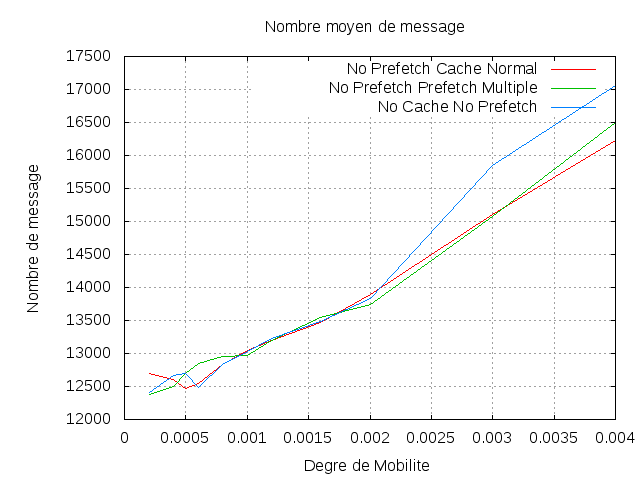
\includegraphics[scale=0.5]{../CacheCode/SolipsisPeersim/resultats/Courbes/Courbes_Final_Rapport/Nombre_Messages_Caches.png}
        \caption{Schéma montrant le nombre de messages}
        \label{courbesNbMessCache:config1}
        \end{figure}

Nous allons maintenant observer la cohérence de la topologie avec les différentes versions du cache (voir figure~\ref{courbesTopoCohCache:config1}). Les différences entre les versions avec cache simple et sans cache sont minimes. Le nombre de cache Hit est pourtant en évolution avec la mobilité. Ces résultats peuvent s'expliquer du fait que si le cache trouve un nœud, la version sans le cache l'aurait peut être aussi fait mais avec l'envoie de messages. Il est possible que si nous augmentions les durées des communications, les résultats soient meilleurs. La fin du stage pourrait permettre de valider ou non cette possibilité.
\par La version du cache fonctionnant avec une recherche renvoyant plusieurs nœuds donne des résultats meilleurs que la version de base (sans cache et sans préchargement). Cette version donne aussi de meilleurs résultats que la version avec un retour simple. Ce résultat est normal, car un plus grand nombre de nœud utile à la cohérence de la topologie est rajouté en un passage.

	\begin{figure}[!h]
        \centering
        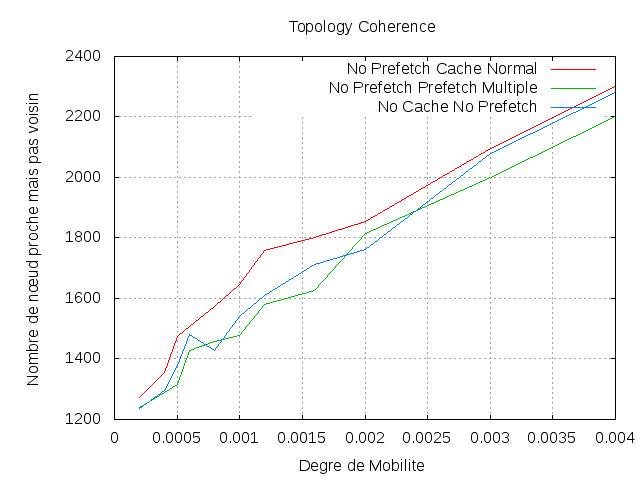
\includegraphics[scale=0.5]{../CacheCode/SolipsisPeersim/resultats/Courbes/Courbes_Final_Rapport/Topology_Coherence_Caches.png}
        \caption{Schéma montrant la cohérence de la topologie}
        \label{courbesTopoCohCache:config1}
        \end{figure}

\subsubsection{Résultats des autres implémentations}

Les mises à jour du cache permettent de récupérer toutes les nouvelles données correspondants aux nœuds stockés. Ces mises à jour permettent donc de moins se tromper entre les coordonnées stockées et les coordonnées effectives des nœuds. Mais cela ne veut pas dire que le cache va permettre de bien meilleurs résultats. En effet, les nœuds mis à jour peuvent avoir beaucoup bougés et donc s'être éloignés du nœud courant. Les tests montrent une augmentation du nombre de messages qui est croissante avec le nombre de nœuds du cache et avec la fréquence du mécanisme de mise à jour. Une très légère amélioration de la cohérence de la topologie apparait et les métriques du cache (nombre de cache Miss, Hit, etc) sont équivalentes à la version sans les mises à jours. Il faudrait tester encore plus de configurations, en faisant des combinaisons avec tous les paramètres pour savoir si le léger gain apparu, peut permettre de combler le surplus de messages.
\par Un autre mécanisme en place permet de contacter un nœud si ses données dans le cache sont considérées comme trop anciennes. Pour évaluer son efficacité, une évaluation du nombre de cache miss réussi et échoué après contact parait judicieuse. Les résultats montrent que le pourcentage de cache Hit se situe au environ de 50\%. Il faut noté que dans les cas où la requête a échoué, elle va tout de même permettre de rafraîchir les données du nœud contacté dans le cache.


\par L'aide aux voisins permet d'économiser un petit nombre de messages, les gains de cette solution sont très peu perceptibles. En moyenne, il a été possible de calculer qu'une requête d'aide réussit environ dans 15\% des cas.

\par Les différents paramètres du cache (taille du cache, limite de distance, limite de temps) peuvent être modifiés et des changements provoquent des différences dans les résultats. L'augmentation des ces paramètres fait perdre en cohérence de la topologie. Lorsque la limite de distance augmente, la fonction de recherche va prendre des nœuds moins intéressant. Mais ce paramètre ne fait pas varier énormément la cohérence de la topologie. En effet la recherche dans la zone de connaissance étant sélectionnée, si la limite de distance est supérieure au rayon de la zone de connaissance, nous ne prendrons pas les nœuds hors de la zone de connaissance. Si nous avions choisi une autre fonction de recherche, ce paramètre aurait impacté plus fortement la cohérence de la topologie.
\par Une augmentation de la limite de temps va provoquer la sélection de nœuds qui ont des valeurs mises à jour il y a longtemps. Ceci est d'autant plus vrai si le mécanisme de mise à jour des données du cache n'est pas activé. Cette augmentation de la limite de temps va ajouter, à l'ensemble des voisins, des nœuds qui pourrait lui être inutiles. La topologie cohérence sera donc moins bonne si on augmente trop la limite de temps. Si nous souhaitons l'augmenter, il faudra activer le mécanisme de contact des nœuds et fixer une autre limite avec une valeur inférieure à la limite de temps.
\par La taille du cache fait varier la longueur des boucles de recherche de nœud. Mais elle modifie que très légèrement sur les résultats si les autres paramètres sont fixés avec des valeurs basses (comme dans les tests). En effet si le cache est grand, il faudra rechercher dans plus de nœuds mais plus de nœuds seront trop vieux pour être pris en compte. De plus si le mécanisme de mise à jour du cache est activé avec un cache de grande taille, le nombre de messages nécessaires sera très grand. Un cache trop grand n'est donc pas utile. De même, un cache trop petit oublierait trop rapidement des nœuds qui auraient pu servir.  

\subsection{Conclusion et perspectives du cache} 

La mise en place du cache permet d'économiser des messages et cela est d'autant plus vrai que la mobilité est grande. Les différents mécanismes mis en place (aide aux voisins, mise à jour du cache, contact d'un nœud) permettent aussi d'améliorer les résultats que ce soit en terme de nombre de messages ou de cohérence de la topologie. D'autres tests pourraient permettre de trouver la meilleure combinaison des différents paramètres, ces tests longs pourraient être réalisés dans le dernier mois du stage. Les deux versions du cache (retour unique ou multiple) permet d'améliorer la cohérence de la topologie. La version à retour multiple est plus efficace car elle permet de rajouter plusieurs nœuds utiles en un seul passage dans le cache.
 
